\documentclass[a4paper, 11pt]{article}
\usepackage[utf8]{inputenc}
\usepackage[left=18mm, right=18mm, top=22mm, bottom=22mm]{geometry}

\usepackage{amsmath,amsfonts,amssymb,bm}
\usepackage[english]{babel}
\usepackage{hyperref}
\usepackage{xcolor}
\usepackage{fancyhdr}
\usepackage{graphicx}
\usepackage{booktabs}
\usepackage{float}
\usepackage{multirow}
\usepackage{caption}
\usepackage{verbatim}  % provides \begin{comment}...\end{comment}

% Preferred style -------------------------------------------------------------
\definecolor{harvardcrimson}{HTML}{8C1D40}
\definecolor{softgrey}{HTML}{F3F3F3}
\definecolor{kwcol}{HTML}{1F4E79}
\definecolor{datablockcol}{HTML}{4B644A}

\hypersetup{
  colorlinks=true,
  linkcolor=harvardcrimson,
  citecolor=harvardcrimson,
  urlcolor=harvardcrimson,
  hypertexnames=false,
}

\pagestyle{fancy}
\fancyhf{}
\rhead{\textcolor{harvardcrimson}{\textbf{clens covariance extensions}}}
\lhead{\textcolor{harvardcrimson}{\textbf{X.\,Tang}}}
\cfoot{\thepage}
\renewcommand{\headrulewidth}{0.4pt}
\renewcommand{\footrulewidth}{0.4pt}
\setlength{\headheight}{14pt}
\renewcommand{\baselinestretch}{1.12}

% Custom commands ------------------------------------------------------------
\newcommand{\lob}{\lambda^{\rm ob}}
\newcommand{\ltr}{\lambda^{\rm tr}}
\newcommand{\zob}{z^{\rm ob}}
\newcommand{\ztr}{z^{\rm tr}}
\newcommand{\hMpc}{h^{-1}\,\mathrm{Mpc}}
\newcommand{\hMsun}{h^{-1}\,M_{\odot}}
\newcommand{\modname}[1]{\textcolor{kwcol}{\texttt{#1}}}
\newcommand{\blk}[1]{\textcolor{datablockcol}{\texttt{#1}}}
\newcommand{\pyfile}[1]{{\small\texttt{#1}}}

\title{\vspace{-4ex}\huge \textbf{Covariance extensions for}\\[0.5ex]
       \Large \textbf{\pyfile{hywu/cluster-lensing-cov} (clens)}}
\author{X.\,Tang}
\date{2026-11-18}

\begin{document}
\maketitle

\begin{abstract}
This document is the technical reference for the six modules under
\pyfile{scripts/} in this fork of
\href{https://github.com/hywu/cluster-lensing-cov}{\pyfile{hywu/cluster-lensing-cov}}
(\modname{clens}). Upstream \modname{clens} computes only the
\emph{Gaussian-field} covariance of a stacked cluster-lensing
$\Delta\Sigma(R)$ (Wu et al.\ 2019, eq.~22: shape noise $+$ uncorrelated
LSS $+$ $(C_\ell^{h\Sigma})^2$); it has no term for the fact that the
$N$ stacked clusters are not identical halos. These scripts add four
independent covariance components on top of that baseline --
halo-to-halo mass/concentration/miscentering scatter
(\modname{intrinsic\_cov.py}), halo ellipticity and orientation
(\modname{halo\_ell\_cov.py}), Poisson-clustered neighbour halos
(\modname{clss\_cov.py}) -- plus a standalone truncated-NFW profile
module (\modname{nfw\_profile.py}) that the first three all build on, a
mean-profile miscentering convolution (\modname{miscentering.py}), and
an alternative HOD-style richness--mass relation with line-of-sight
projection (\modname{hod\_richness.py}) that can replace \modname{clens}'s
default log-normal $P(\lambda\mid M)$ via a one-line monkeypatch. All
five covariance components are returned as a common
\modname{CovStackedDeltaSigma} container that merges, sums, and
plots them consistently. This document does \emph{not} cover
\pyfile{notebooks/run\_cov\_clens.ipynb} or the upstream
\pyfile{clens/} package itself, only the added scripts.
\end{abstract}

\tableofcontents
\vspace{1em}

% ============================================================================
\section{How the pieces fit together}
\label{sec:topology}

\begin{center}
\fbox{\parbox{0.95\linewidth}{\centering
\modname{clens.CovDeltaSigma} (\texttt{cov\_stat}) $\ \oplus\ $
\modname{IntrinsicCov} (\texttt{cov\_lambdaM}, \texttt{cov\_cM},
\texttt{cov\_miscen}) $\ \oplus\ $
\modname{HaloEllCov} (\texttt{cov\_ell}) $\ \oplus\ $
\modname{CLSSCov} (\texttt{cov\_clss})
$\ \xrightarrow{\texttt{.merge()}}\ $
\modname{CovStackedDeltaSigma}}}
\end{center}

Each of the three covariance calculators (\modname{IntrinsicCov},
\modname{HaloEllCov}, \modname{CLSSCov}) is constructed once per
$(z,\lambda)$ bin from a \modname{clens} cosmology \blk{co} and scaling
relation \blk{sr}, exposes a \texttt{calc\_cov(rp\_edges, N, cov\_stat)}
method that must be called with the \emph{same} radial binning and
cluster count $N$ used for the upstream
\texttt{clens.CovDeltaSigma.calc\_cov}, and returns a
\modname{CovStackedDeltaSigma} (\S\ref{sec:container}) holding its own
component(s) plus the \texttt{cov\_stat} it was passed. Calling
\texttt{.merge()} on any one of these with the others combines every
component into a single object, after checking that the radial
binning, $z$ bin, $\lambda$ bin and any component shared between two
inputs agree. \modname{nfw\_profile.NfwProfile} underlies
\modname{IntrinsicCov}'s per-halo profile sampling as well as all of
\modname{HaloEllCov} and \modname{CLSSCov} (both need the analytic
projected-cylinder mass of a truncated NFW halo, at a different
radius than the one it is centred on). \modname{miscentering.py} is
\emph{not} part of this merge graph: it acts on the stacked
\emph{mean} profile (for comparing, e.g., ``HOD'' vs ``HOD +
miscentering'' curves), not on a covariance matrix -- the miscentering
contribution to the \emph{covariance} is \texttt{cov\_miscen} inside
\modname{IntrinsicCov} (\S\ref{sec:miscen-cov}). The two models move
in lock-step ($f_{\rm mis}, \tau$, and the same Gamma-offset
population) but compute different things.

% ============================================================================
\section{\pyfile{nfw\_profile.py} -- analytic (truncated) NFW profile}
\label{sec:nfw}

\modname{Path}\ \pyfile{scripts/nfw\_profile.py} (\texttt{NfwProfile}).
Ported from
\href{https://github.com/estevesjh/CLensPy}{CLensPy} (\texttt{clenspy/halo/nfw.py},
MIT licence, reproduced in the file header) so that \modname{cov\_clens}
does not depend on the CLensPy package; everything below the
\emph{cov\_clens additions} marker in the source is new.

\paragraph{Mass definition.} The class carries no cosmology: the
caller passes the reference density \texttt{rho\_ref} that closes
$M_{200} = 200\,\rho_{\rm ref}\,\tfrac{4}{3}\pi r_{200}^3$ (comoving
mean matter density $\Rightarrow M_{200m}$, which is what every script
in this fork uses, matching \modname{clens}'s own halo mass
definition). The 3D profile is the usual
\begin{equation}
  \rho(r) = \frac{\rho_s}{x(1+x)^2}, \qquad x = r/r_s, \qquad
  \rho_s = \frac{M_{200}}{4\pi r_s^3\left[\ln(1+c) - c/(1+c)\right]},
\end{equation}
with $r_s = r_{200}/c_{200}$. The upstream methods (\texttt{density},
\texttt{fourier}, \texttt{sigma}, \texttt{mean\_sigma},
\texttt{deltasigma}) implement the standard untruncated closed forms
(Wright \& Brainerd 2000 for $\Sigma,\Delta\Sigma$); each piecewise
kernel is regularised at its $x=1$ kink with a pre-computed Taylor
series (\texttt{\_F\_SERIES}, \texttt{\_G\_SERIES}, 9 terms) to avoid
the $0/0$ cancellation of the direct closed form within
$|x-1|<10^{-2}$, and \texttt{\_gbarNfw} is evaluated from its own
closed form (not reconstructed as $f + g/2$, which loses every digit
below $x\sim 10^{-6}$) with a small-$x$ series below $x = 3\times
10^{-3}$.

\paragraph{Added: truncation at $r_{200}$.} Every halo used by
\modname{IntrinsicCov}, \modname{HaloEllCov} and \modname{CLSSCov} is
truncated ($\rho \equiv 0$ for $r > r_{200}$), so its projected mass
converges and equals exactly $M_{200}$ outside $r_{200}$ -- required
for \modname{HaloEllCov}'s ellipsoidal projection
(\S\ref{sec:halo-ell}) and for \modname{CLSSCov}'s neighbour-halo
profiles (\S\ref{sec:clss}), both of which need the cylinder mass
$M_{2D}(<R)$ evaluated at radii that can be \emph{larger} than
$r_{200}$ of a small neighbour halo. The truncated surface density
(Takada \& Jain 2003, eq.~27) is
\begin{equation}
  \Sigma(R) = 2 r_s \rho_s\, F(X), \qquad X = R/r_s \le c,
\end{equation}
\begin{equation}
  F(X) = -\frac{\sqrt{c^2-X^2}}{(1-X^2)(1+c)}
         + \frac{1}{(1-X^2)^{3/2}}\,
           \operatorname{arccosh}\frac{X^2+c}{X(1+c)} \qquad (X<1),
\end{equation}
continued to $X>1$ via $\operatorname{arccosh}\to-\arccos$,
$(1-X^2)^{3/2}\to(X^2-1)^{3/2}$, and linearly interpolated across the
$0/0$ kink at $X=1$ from $X = 1\mp10^{-3}$. The truncated projected
cylinder mass is derived by subtracting, from $M_{200}$, the mass of
every shell $r>X$ that lies outside the cylinder:
\begin{equation}
\label{eq:m2d}
  M_{2D}(<R) = M_{200} - 4\pi\rho_s r_s^3\, J(X), \qquad
  J(X) = \int_X^c \frac{\sqrt{t^2-X^2}}{(1+t)^2}\,dt,
\end{equation}
which (integration by parts, then $t = X\cosh\theta$, $\tau =
\tanh(\theta/2)$) has the closed form
\begin{equation}
  J = -\frac{\sqrt{c^2-X^2}}{1+c} + \operatorname{arccosh}\frac{c}{X}
      - K, \qquad
  \tau_c = \sqrt{\frac{c-X}{c+X}},
\end{equation}
\begin{equation}
  K = \begin{cases}
     \dfrac{2}{\sqrt{1-X^2}}\,\operatorname{arctanh}\!\Big(\tau_c
        \sqrt{\tfrac{1-X}{1+X}}\Big), & X<1 \\[2mm]
     \tau_c, & X=1 \\[1mm]
     \dfrac{2}{\sqrt{X^2-1}}\,\arctan\!\Big(\tau_c
        \sqrt{\tfrac{X-1}{X+1}}\Big), & X>1,
     \end{cases}
\end{equation}
with a dedicated small-$X$ series ($X<10^{-3}$, where the two
logarithms inside $J$ cancel) built from $\bar g(X)$:
\begin{equation}
  M_{2D} = 2\pi\rho_s r_s^3 X^2\Big[\bar g(X) - \ln\tfrac{1+c}{c}
           + \tfrac{1}{1+c}\Big] + O(X^4).
\end{equation}
\texttt{mass\_2d(R, truncated=True)} returns $M_{200}$ for $R\ge
r_{200}$ and Eq.~\eqref{eq:m2d} otherwise, broadcasting over an
arbitrary halo shape and an arbitrary-rank radius array via
\texttt{\_halo\_axes} (every per-halo quantity is reshaped with one
trailing singleton axis per axis of \texttt{R}).

% ============================================================================
\section{\pyfile{miscentering.py} -- mean-profile offset convolution}
\label{sec:miscen-mean}

\modname{Path}\ \pyfile{scripts/miscentering.py}
(\texttt{sigma\_and\_deltasigma}, \texttt{miscentered\_DeltaSigma},
\texttt{R\_lambda\_comoving}). Model: McClintock et al.\ 2019 \S5.2;
offset-population prior: Zhang et al.\ 2019 (arXiv:1901.07119),
$\rho = 0.835 \Rightarrow f_{\rm mis}=0.165$, $\tau=0.166$ (close to,
but not identical to, the Table~1 central values used elsewhere in
this fork's mock pipelines). \texttt{sigma\_and\_deltasigma} first
recovers $\Sigma_{\rm cen}(R)$ and $\Delta\Sigma_{\rm cen}(R)$ from a
\modname{clens} \texttt{LensingProfiles} object directly (its own
\texttt{calc\_Sigma} is broken upstream -- it still references a
removed \texttt{self.nu}), by reusing the halo-matter correlation
function already computed for $\Delta\Sigma$.

The azimuthally averaged surface density at projected radius $R$ seen
with the finder's centre offset by $R_{\rm mis}$ from the true centre
is the angular convolution
\begin{equation}
  \Sigma_{\rm mis}(R\mid R_{\rm mis}) = \frac{1}{2\pi}
    \int_0^{2\pi} \Sigma_{\rm cen}\!\left(
      \sqrt{R^2+R_{\rm mis}^2+2RR_{\rm mis}\cos\phi}\right)d\phi,
\end{equation}
evaluated in log-log-interpolated $\Sigma_{\rm cen}$ and averaged over
the offset population
\begin{equation}
  P(x\mid\tau) = \frac{x}{\tau^2}\,e^{-x/\tau}, \qquad
  x \equiv R_{\rm mis}/R_\lambda, \qquad
  R_\lambda(\lambda,z) = \left(\frac{\lambda}{100}\right)^{0.2}
    \hMpc\ \text{(physical)},
\end{equation}
(\texttt{R\_lambda\_comoving} converts this to $h$-free comoving Mpc
to match \modname{clens}'s internal units). $\Delta\Sigma_{\rm mis}$
is \emph{not} the same convolution applied to $\Delta\Sigma_{\rm
cen}$ -- it is re-derived from the convolved $\Sigma_{\rm mis}$ via the
usual mean-enclosed-density definition (trapezoidal in $R\,dR$,
\texttt{\_delta\_sigma}), and the observed stack mixes the two
populations:
\begin{equation}
  \Delta\Sigma_{\rm obs}(R) = (1-f_{\rm mis})\,\Delta\Sigma_{\rm cen}(R)
    + f_{\rm mis}\,\Delta\Sigma_{\rm mis}(R).
\end{equation}
This is the quantity plotted as the ``HOD + miscentering'' curve in
\pyfile{notebooks/run\_cov\_clens.ipynb}; by construction it leaves
the \emph{covariance} unchanged (miscentering shifts the mean, the
scatter in \emph{which} clusters are offset is a separate,
covariance-level effect -- \S\ref{sec:miscen-cov}).

% ============================================================================
\section{\pyfile{intrinsic\_cov.py} -- halo-to-halo scatter}
\label{sec:intrinsic}

\modname{Path}\ \pyfile{scripts/intrinsic\_cov.py}
(\texttt{IntrinsicCov}, \texttt{CovStackedDeltaSigma}). Method:
McClintock et al.\ 2019 \S3.2.4 (the DES~Y1 semi-analytic covariance's
treatment of mass--richness scatter and miscentering, by sampling the
halo population). \modname{clens} stacks $N$ clusters and computes
only the Gaussian-field covariance of their \emph{mean} profile; it
has no term for the fact that those $N$ halos do not share one
profile. This module adds that term via the law of total covariance,
\begin{equation}
\label{eq:cov-intr}
  \mathrm{Cov}_{\rm intr}(R_i,R_j) = \frac{1}{N}\Big[
    \mathbb{E}_{\rm pop}(\Delta\Sigma_i\Delta\Sigma_j)
    - \mathbb{E}_{\rm pop}(\Delta\Sigma_i)\,\mathbb{E}_{\rm pop}(\Delta\Sigma_j)
  \Big],
\end{equation}
with $\mathbb{E}_{\rm pop}$ weighted by $dn/d\ln M\times P(\lambda\in
{\rm bin}\mid M)$ and the miscentering mixture $(1-f_{\rm
mis})\,\delta(R_{\rm mis}) + f_{\rm mis}\,\mathrm{Gamma}(x\mid\tau)$,
decomposed into three nested pieces (mass $\to$ concentration $\to$
offset):
\begin{align}
  \texttt{cov\_lambdaM}  &= \mathrm{Cov}_M\big[\mathbb{E}(\Delta\Sigma\mid M)\big]/N
    &&\text{(mass spread in the richness bin)}, \\
  \texttt{cov\_cM}       &= \mathbb{E}_M\big[\mathrm{Cov}_c\big(\mathbb{E}(\Delta\Sigma\mid M,c)\big)\big]/N
    &&\text{(concentration scatter at fixed $M$)}, \\
  \texttt{cov\_miscen}   &= \mathbb{E}_{M,c}\big[\mathrm{Cov}_{\rm mis}(\Delta\Sigma\mid M,c)\big]/N
    \label{eq:miscen-cov-term}
    &&\text{(offset draws at fixed $M,c$),}
\end{align}
which sum exactly to Eq.~\eqref{eq:cov-intr} (the split into three
depends on the $M\to c\to$ offset nesting order, the total does not).
Each halo's profile is the \modname{clens} 1-halo (truncated NFW,
\S\ref{sec:nfw}) plus linear 2-halo term, $\max(1h,2h)$, but with the
NFW concentration drawn from a $c(M)$ relation instead of fixed at
the median: by default the Duffy et al.\ 2008 $c_{200m}(M,z)$ relation
(\texttt{cM='duffy08'}; \texttt{cM='correa'} reproduces \modname{clens}'s
own default),
\begin{equation}
  c_{200m}(M,z) = A\left(\frac{M}{M_{\rm pivot}}\right)^{\!B}(1+z)^C,
  \qquad M_{\rm pivot} = 2\times10^{12}\,\hMsun,
\end{equation}
with full-sample Table~1 values $(A,B,C) = (10.14,\,-0.081,\,-1.01)$
for $\Delta=200m$ ($0<z<2$), and a log-normal scatter
$\sigma_{\ln c}\approx 0.15\ln 10\approx 0.35$ (from the reported
$\sigma_{\log_{10}c}\sim 0.15$), integrated with Gauss--Hermite
quadrature in $\ln c$ ($n_c$ nodes; \texttt{include\_concentration=False}
collapses this to the median $c(M)$ only, dropping \texttt{cov\_cM}).
\texttt{calc\_profiles} evaluates every draw on an $(n_M, n_c, 1+n_{\rm
mis}, n_{rp})$ grid (index 0 of the offset axis is the centred
profile) and \texttt{calc\_cov} contracts it with
\texttt{numpy.einsum} into the three terms of
Eq.~\eqref{eq:miscen-cov-term}.

\subsection{The \texttt{CovStackedDeltaSigma} container}
\label{sec:container}

A frozen dataclass holding one $(z,\lambda)$ bin's radial grid
(\texttt{R\_hiMpc}, comoving $\hMpc$) and up to six named covariance
components (\texttt{cov\_stat}, \texttt{cov\_cM},
\texttt{cov\_lambdaM}, \texttt{cov\_miscen}, \texttt{cov\_ell},
\texttt{cov\_clss}, every one in $(h\,M_\odot/\mathrm{pc}^2)^2$),
plus optionally the population-mean \texttt{DeltaSigma}. On
construction, every supplied component is validated: correct shape
$(n,n)$, symmetric, and positive semi-definite (smallest eigenvalue
$\ge -10^{-10}\times$ its own max $|C|$), then made read-only.
\texttt{from\_clens} converts \modname{clens}'s $h$-free comoving
Mpc / $M_\odot\,\mathrm{pc}^{-2}$ convention to this container's
$h$-unit one. \texttt{merge} combines the components from several
calculators run on the same bin and radial grid, raising if a
component present in more than one input disagrees beyond floating
tolerance; \texttt{total(include=...)} sums a chosen subset (default:
everything present); \texttt{frac\_diag()} gives each component's
share of the total variance at each $R$; \texttt{save}/\texttt{load}
round-trip through a single \texttt{.npz}.

% ============================================================================
\section{\pyfile{halo\_ell\_cov.py} -- halo ellipticity \& orientation}
\label{sec:halo-ell}

\modname{Path}\ \pyfile{scripts/halo\_ell\_cov.py}
(\texttt{HaloEllCov}, \texttt{ell\_profiles},
\texttt{bin\_subgrid}, \texttt{binned\_ds\_from\_mcyl}). Gruen, Seitz,
Becker, Friedrich \& Mana 2015 (MNRAS 449, 4264; arXiv:1501.01632),
\S3.2.4, eqs.~27--31: real halos are not spherical, and stacking
randomly oriented triaxial halos adds covariance even to an
otherwise-identical population. Modelled as a prolate NFW with
volume-preserving ellipsoidal radius ($z'$ = long axis)
\begin{equation}
  r_e^2 = \mathbf{x}^T A\,\mathbf{x}, \qquad
  A = \mathrm{diag}\big(q^{-2/3},\,q^{-2/3},\,q^{4/3}\big),
\end{equation}
axis ratio $q\sim\mathcal N(0.6,0.12)$ truncated to $[q_{\rm min},1]$
(Bett et al.\ 2007, $\sim10^{14}\,M_\odot$ halos) and isotropic
orientation, $\cos\alpha\sim U[0,1]$. The covariance is the scatter
over shape and orientation at fixed mass,
\begin{equation}
  C^{\rm ell}_{ij} = \mathbb{E}_{q,\alpha}
    \big[\Delta\Sigma_i\,\Delta\Sigma_j\big]
    - \mathbb{E}_{q,\alpha}[\Delta\Sigma_i]\,\mathbb{E}_{q,\alpha}[\Delta\Sigma_j],
\end{equation}
calibrated on simulations with amplitude $c_{\rm ell}=3.7\pm0.3$
($z=0.25$; $c_{\rm ell}=1$ is the pure analytic model).

For any ellipsoidal $\rho(r_e)$, the exact projected surface density
along line of sight $\mathbf n=(\sin\alpha,0,\cos\alpha)$ is
$\Sigma(R)=\Sigma_{\rm sph}(\xi)/\sqrt{\mathbf n^T\!A\,\mathbf n}$,
$\xi^2=\mathbf R^T B\,\mathbf R$ with $B=\mathrm{diag}\big(q^{2/3}/
(\mathbf n^T\!A\,\mathbf n),\,q^{-2/3}\big)$ in the sky basis, where
$\Sigma_{\rm sph}$ is the projection of the \emph{spherical} profile
(so projected mass is conserved and $\Sigma_{\rm sph}$ is the analytic
truncated-NFW \texttt{sigma\_truncated}, \S\ref{sec:nfw}); only the
1-halo term is elliptical, the identical spherical 2-halo term cancels
in the covariance. Azimuthally averaging the tangential shear over an
annulus needs only the cylinder mass, closed-form up to one smooth
angular average,
\begin{equation}
  M_{\rm cyl}(<R) = \frac{1}{\sqrt{\mathbf n^T\!A\,\mathbf n}}\,
    \Big\langle \frac{M_{2D}\big(<R\,s(\phi)\big)}{s(\phi)^2}
    \Big\rangle_\phi, \qquad
  s^2(\phi) = B_{11}\cos^2\phi + B_{22}\sin^2\phi,
\end{equation}
($M_{2D}$ the truncated-NFW cylinder mass, Eq.~\ref{eq:m2d}), evaluated
in one broadcast over (mass, $q$, $\alpha$, $R$, sub-annulus,
quarter-period $\phi$) -- no Python loops (\texttt{ell\_profiles}).
\texttt{binned\_ds\_from\_mcyl} converts $M_{\rm cyl}(R)$ on a
log-spaced sub-grid per annulus (\texttt{bin\_subgrid}) into the
annulus-averaged tangential $\Delta\Sigma$,
\begin{equation}
  \langle\Delta\Sigma\rangle_{\rm bin} =
    \frac{2\!\int M_{\rm cyl}\,d\ln R - \big[M_{\rm cyl}(R_2)-M_{\rm cyl}(R_1)\big]}
         {\pi\left(R_2^2-R_1^2\right)}.
\end{equation}
The within-mass variance is averaged over the bin's mass distribution
only (Gauss--Legendre in $q,\alpha$; the scatter \emph{between} masses
is \texttt{intrinsic\_cov.py}'s \texttt{cov\_lambdaM}):
\begin{equation}
  \texttt{cov\_ell} = c_{\rm ell}\,
    \mathbb{E}_M\big[\mathrm{Cov}_{q,\alpha}(\Delta\Sigma\mid M)\big]\,/\,N.
\end{equation}

% ============================================================================
\section{\pyfile{clss\_cov.py} -- correlated LSS (Poisson neighbours)}
\label{sec:clss}

\modname{Path}\ \pyfile{scripts/clss\_cov.py}
(\texttt{CLSSCov}, \texttt{projected\_corr}, \texttt{offset\_nodes},
\texttt{offset\_profiles}). Gruen et al.\ 2015 \S3.2.2, eqs.~22--26:
the number of neighbouring halos clustered around the cluster is
Poisson, $\mathrm{Cov}(\lambda_k,\lambda_l)=\delta_{kl}\langle
\lambda_k\rangle$, giving a covariance contribution
\begin{equation}
  C^{\rm corr}_{ij} = \int dP_c(h)\,\Delta\Sigma_i(h)\,\Delta\Sigma_j(h), \qquad
  dP_c = b(M_{\rm cl})\,b(M)\,n(M)\,d\ln M\;\, w_p(R_{\rm off})\,2\pi R_{\rm off}\,dR_{\rm off},
\end{equation}
\begin{equation}
  w_p(R) = \int_{-\Pi}^{\Pi}\xi_{\rm lin}\big(\sqrt{R^2+\chi^2}\big)\,d\chi,
  \qquad \Pi = 200\,\hMpc,
\end{equation}
counting only the \emph{excess} (correlated) neighbours -- the
uncorrelated ``$1$'' of $1+\xi$ is the uncorrelated LSS already in
\modname{clens}'s Gaussian covariance, and $b(M_{\rm cl})$ is the
richness bin's mean halo bias (so $C^{\rm corr}$ is linear in it,
\texttt{self.b\_cl}). Unlike \texttt{cov\_ell}/\texttt{cov\_lambdaM},
no mean is subtracted (this is a Poisson count, not a scatter about a
mean); calibrated on simulations with $c_{\rm corr}=5.0\pm0.3$
($z=0.25$; $4.2\pm1.1$ at $z=0.5$; $c_{\rm corr}=1$ is the analytic
lower limit, since Gruen+15 report the analytic term omits 3-point
terms).

Each neighbour contributes the annulus-averaged tangential
$\Delta\Sigma_t(R) = M_{\rm cyl}(<R)/(\pi R^2) - \Sigma_{\rm ring}(R)$
of one truncated NFW halo (Duffy+08 median $c(M)$, no scatter -- the
scatter machinery lives in \texttt{intrinsic\_cov.py}) seen at
projected offset $d$ from the cluster centre. The cylinder mass of an
\emph{offset} halo, by parts in $f(s)=\arccos\!\big[(s^2+d^2-R^2)/
(2sd)\big]/\pi$ (the fraction of the halo's ring at radius $s$ inside
the cluster-centred circle of radius $R$), is
\begin{equation}
  M_{\rm cyl}(R;d) = \int_a^b M_{2D}(<s)\,\big(-f'(s)\big)\,ds,
  \qquad a=|R-d|,\ b=R+d,
\end{equation}
regularised against the endpoint singularities of $f'$ by substituting
$s = a + \tfrac12(b-a)(1-\cos\theta)$,
\begin{equation}
  M_{\rm cyl}(R;d) = \frac{1}{\pi}\int_0^\pi
    \frac{M_{2D}(s)\,\big(s^2-d^2+R^2\big)}{s\,\sqrt{(s+a)(s+b)}}\,d\theta
  \quad(\texttt{offset\_profiles}),
\end{equation}
and evaluated with Gauss--Legendre quadrature in $\theta$ for a vector
of neighbour masses and offsets at once. The offset nodes
(\texttt{offset\_nodes}) are Gauss--Legendre in $\ln d$, with annulus
edges as panel breakpoints (a small halo's binned $\Delta\Sigma_t(d)$
has a kink wherever $d$ crosses an annulus edge). Combining both
integrals over the Tinker08/Tinker10 neighbour mass function and bias
(\texttt{HaloStat}) gives
\begin{equation}
  \texttt{cov\_clss} = c_{\rm corr}\,b_{\rm cl}
    \int d\ln M\; b(M)\,\frac{dn}{d\ln M}
    \int 2\pi R_{\rm off}\,dR_{\rm off}\; w_p(R_{\rm off})\,
    \Delta\Sigma_i\,\Delta\Sigma_j \,\Big/\, N,
\end{equation}
with the per-mass contribution kept in \texttt{self.dcov\_dlnM} before
the $\ln M$ integral, so \texttt{cov\_clss =
c\_corr * trapz(dcov\_dlnM, lnM) / N} exactly.

% ============================================================================
\section{\pyfile{hod\_richness.py} -- HOD richness--mass relation}
\label{sec:hod}

\modname{Path}\ \pyfile{scripts/hod\_richness.py}
(\texttt{HODRichness}, \texttt{enable\_hod\_hook}). Replaces
\modname{clens}'s default log-normal $P(\ln\lambda\mid M)$ with the
halo-occupation model of Costanzi et al.\ 2026 (C26, arXiv:2604.05833)
\S\,III, eq.~15, plus the Costanzi et al.\ 2019 (C19, arXiv:1807.07072)
eq.~6 line-of-sight projection kernel -- the same two models used in
this user's Buzzard mock pipeline
(\pyfile{mocks/mock\_cluster\_buzzard}), but evaluated here
\emph{analytically} (as a bin probability $P(\lob\in{\rm bin}\mid
M,z)$) rather than by Monte Carlo sampling, since \modname{clens}
needs a selection \emph{function}, not per-halo draws.

\paragraph{Intrinsic richness.} $\ltr = \lambda_{\rm cen}+\lambda_{\rm
sat}$, $\lambda_{\rm cen}=\mathbb{1}[M\ge M_{\rm min}]$, mean satellite
count
\begin{equation}
  \bar\lambda_{\rm sat}(M,z) = \left(\frac{M-M_{\rm min}}{M_1-M_{\rm min}}\right)^{\!\alpha}
    \left(\frac{1+z}{1+z_\star}\right)^{\!\epsilon},
\end{equation}
clipped to 0 below $M_{\rm min}$, with default C26 mock values
$\log_{10}M_{\rm min}=11.4$, $\log_{10}M_1=12.7$ [$\hMsun$, $M_{200m}$],
$\alpha=0.86$, $\epsilon=0.28$, $\sigma_\lambda=0.185$, $z_\star=0.45$.
Rather than drawing an integer satellite count per halo,
\texttt{p\_bin} sums the Poisson probability mass function over the
satellite count $n$ directly (\texttt{gammaln}-stabilised, truncated
at $n_{\max}=\bar\lambda_{\rm sat}+n_{\rm pad}\sqrt{\bar\lambda_{\rm
sat}+1}+20$), broadening each Poisson rate with the C26 super-Poisson
scatter $w_{\rm intr}=\max(\sigma_\lambda\,\bar\lambda_{\rm sat},
10^{-6})$ before convolving with the C19 projection kernel.

\paragraph{Projection kernel.} Identical construction to this fork's
Buzzard mock (\pyfile{mocks/mock\_cluster\_buzzard/docs/MockDataVector.tex}
\S3): a Gaussian-core $+$ exponentially-modified-Gaussian (EMG) tail
mixture,
\begin{equation}
  P(\lob\mid\ltr,z) = (1-f_{\rm prj})\,\mathcal N(\mu,\sigma)
    + f_{\rm prj}\,\mathrm{EMG}(\mu,\sigma,\tau),
\end{equation}
with $(\mu,\sigma,\tau,f_{\rm prj})$ functions of $\ltr$ via
coefficients linearly interpolated across the same 15 redshift knots
($z=0.10,\dots,0.80$) of
\pyfile{scripts/prj\_params\_DESY3\_lss\_lin\_dep\_getdist\_v1.txt}.
\texttt{\_p\_bin\_obs} evaluates the closed-form bin probability
$P(\lambda_{\min}\le\lob<\lambda_{\max}\mid\ltr,z)$ directly from the
Gaussian and EMG CDFs (\texttt{scipy.stats.norm}, \texttt{exponnorm}),
folding the intrinsic scatter $w_{\rm intr}$ into the Gaussian core's
effective width $\sigma_{\rm eff}=\sqrt{\sigma_{\rm pr}^2 +
(b_\mu\,w_{\rm intr})^2}$ (exact for the Gaussian branch since
$\mu(\ltr)$ is linear in $\ltr$; an approximation for the EMG branch,
good while $w_{\rm intr}\ll\ltr$, i.e.\ away from the $M\sim M_{\rm
min}$ threshold). \texttt{use\_projection=False} recovers the
pre-projection bin probability on the true richness alone.

\paragraph{Wiring into \modname{clens}.} \modname{clens}'s
\texttt{RichnessSelection.lnM\_selection} method (which every halo-mass
function/bias/lensing integral calls to get $P(\lambda\in{\rm
bin}\mid M,z)$) is monkeypatched by \texttt{enable\_hod\_hook()}: if
the scaling relation object passed to \modname{clens} exposes a
\texttt{p\_bin} method (as \texttt{HODRichness} does), that is called
instead of the original log-normal selection; log-normal scaling
relations (no \texttt{p\_bin}) are unaffected and fall through to the
original implementation. This one hook changes counts, bias (hence
every covariance term above) and the mean profile consistently
wherever \modname{clens} or this fork's calculators query the
selection function -- no other code change is needed to switch the
whole pipeline from the C21 log-normal default to the HOD model.

% ============================================================================
\section{Combined output}
\label{sec:combined}

\begin{figure}[H]
\centering
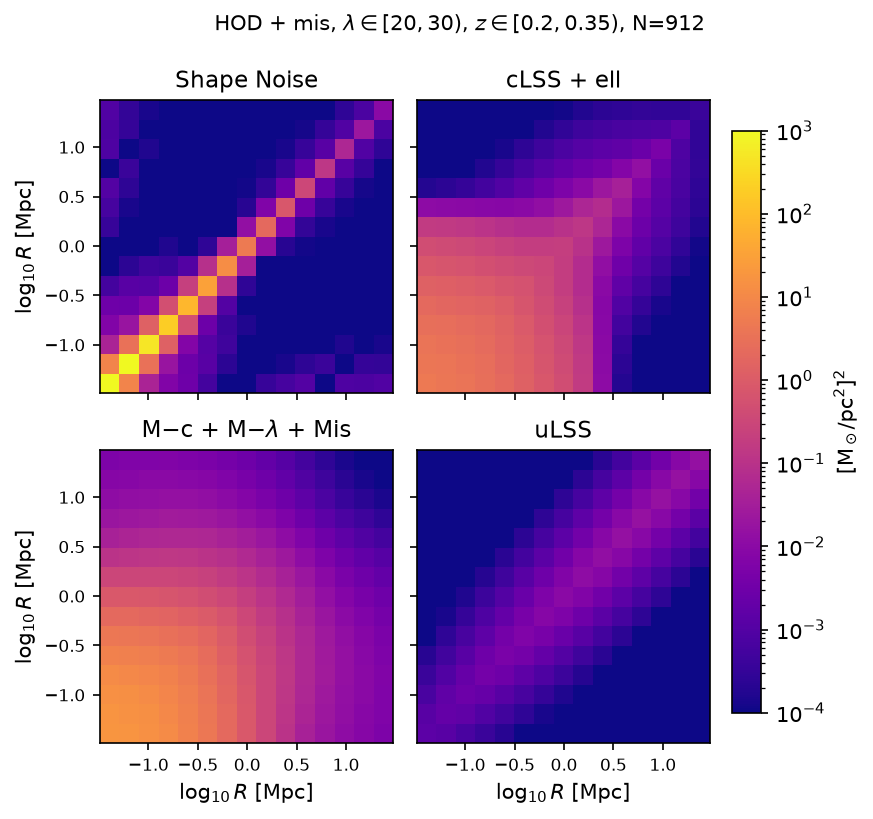
\includegraphics[width=0.85\linewidth]{../plots/cov_stacked_components.png}
\caption{\texttt{CovStackedDeltaSigma.components()} for one
$(\lambda,z)$ bin with the HOD richness relation
(\S\ref{sec:hod}) and $f_{\rm mis}=0.165$, $\tau=0.166$
(\S\ref{sec:miscen-mean}--\ref{sec:intrinsic}): the DES~Y1-style
2$\times$2 panel grid (McClintock+19 Fig.~6 layout) groups
\texttt{cov\_stat}'s shape-noise and uncorrelated-LSS pieces against
the mass--concentration--miscentering intrinsic terms
(\S\ref{sec:intrinsic}) and the halo-ellipticity + correlated-LSS
terms (\S\ref{sec:halo-ell}--\ref{sec:clss}), produced by
\texttt{run\_cov\_clens.ipynb} after \texttt{merge}-ing all four
calculators.}
\label{fig:stacked-components}
\end{figure}

\begin{figure}[H]
\centering
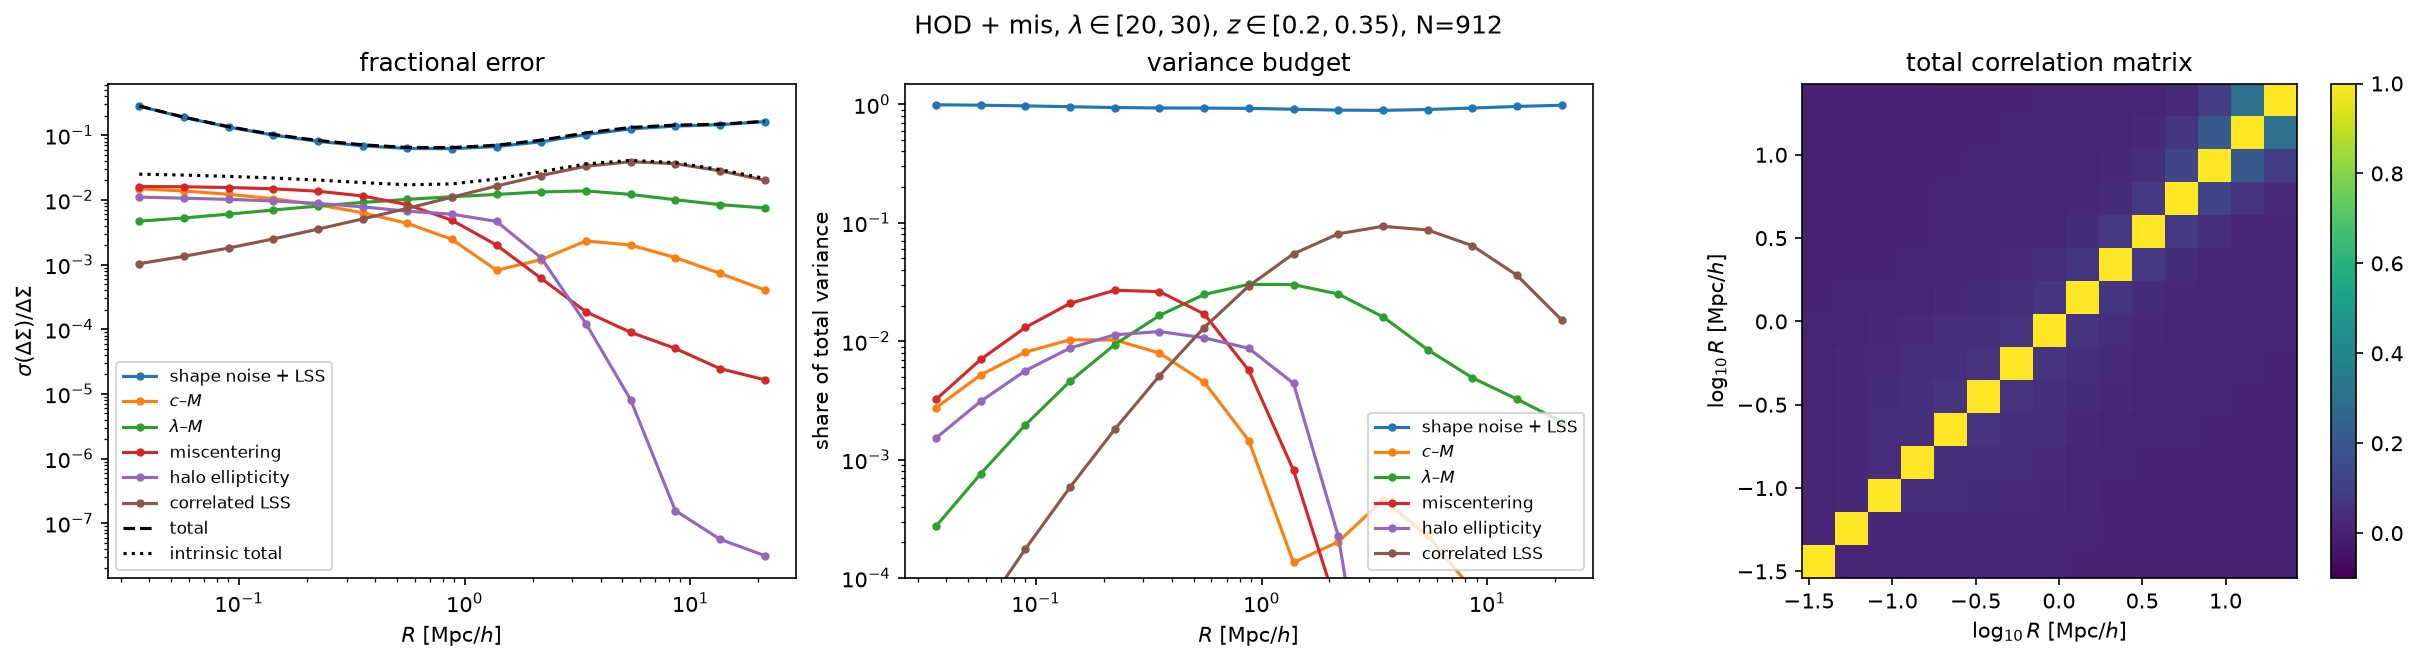
\includegraphics[width=0.95\linewidth]{../plots/cov_stacked_budget.png}
\caption{Fractional error and variance budget
(\texttt{CovStackedDeltaSigma.frac\_diag()}) of every component in
Fig.~\ref{fig:stacked-components}, plus the total correlation matrix.
At small $R$ the halo-to-halo mass/concentration/miscentering scatter
of \S\ref{sec:intrinsic} dominates over \modname{clens}'s own Gaussian
shape-noise term; at large $R$ the Gaussian uncorrelated-LSS term
dominates.}
\label{fig:stacked-budget}
\end{figure}

% ============================================================================
\section{Known simplifications and provenance notes}
\label{sec:notes}

\begin{itemize}
  \setlength\itemsep{2pt}
  \item \textbf{\texttt{NfwProfile} is a verbatim port}, not a
    reimplementation -- see the licence header in
    \pyfile{scripts/nfw\_profile.py}. Only the truncated
    \texttt{sigma\_truncated}/\texttt{mass\_2d} pair and the
    scalar/array-shape bookkeeping around them are new.
  \item \textbf{Concentration--mass relation default.} All three
    covariance calculators default to \texttt{cM='duffy08'}
    (Duffy et al.\ 2008), not \modname{clens}'s own default
    (\texttt{cM='correa'}, Correa et al.); pass \texttt{cM='correa'}
    to reproduce \modname{clens}'s internal concentration exactly,
    at the cost of losing the published Duffy+08 scatter
    $\sigma_{\log_{10}c}\sim0.15$ used for \texttt{cov\_cM}.
  \item \textbf{Amplitude parameters $c_{\rm ell}$, $c_{\rm corr}$ are
    simulation-calibrated, not Buzzard- or \modname{clens}-calibrated.}
    Gruen et al.\ 2015 report $c_{\rm ell}=3.7\pm0.3$ and
    $c_{\rm corr}=5.0\pm0.3$ at $z=0.25$ from their own simulations;
    both default to those values here with no independent check
    against this fork's halo catalogue.
  \item \textbf{\texttt{cov\_miscen} vs.\ the mean-profile
    miscentering of \S\ref{sec:miscen-mean} share parameters but not
    code}: \texttt{IntrinsicCov} samples the offset population on its
    own \texttt{n\_mis}-node grid inside \texttt{calc\_profiles}
    (needed because it must also vary $M$ and $c$ on the same grid),
    while \texttt{miscentering.py} convolves the already-stacked mean
    profile directly. Keep $f_{\rm mis}$, $\tau$ consistent between
    the two if comparing a mean-profile shift against its covariance
    contribution.
  \item \textbf{\texttt{HODRichness} is evaluated analytically}, in
    contrast to the Buzzard mock's Monte Carlo sampler of the same
    C26/C19 model (\pyfile{mocks/mock\_cluster\_buzzard}): this module
    must return a smooth bin-probability function because
    \modname{clens}'s mass-function and bias integrals need
    $P(\lambda\in{\rm bin}\mid M,z)$ evaluated at arbitrary $M$, not a
    finite halo sample.
\end{itemize}

% ============================================================================
\section{File map}
\label{sec:files}

\begin{itemize}
  \setlength\itemsep{1pt}
  \item \pyfile{scripts/nfw\_profile.py} -- \S\ref{sec:nfw}: analytic
    (truncated) NFW profile, shared by the three calculators below.
  \item \pyfile{scripts/miscentering.py} -- \S\ref{sec:miscen-mean}:
    offset-convolution miscentering of the stacked \emph{mean}
    profile.
  \item \pyfile{scripts/intrinsic\_cov.py} -- \S\ref{sec:intrinsic}:
    halo-to-halo mass/concentration/miscentering covariance
    (\texttt{IntrinsicCov}) and the shared
    \texttt{CovStackedDeltaSigma} container.
  \item \pyfile{scripts/halo\_ell\_cov.py} -- \S\ref{sec:halo-ell}:
    halo ellipticity + orientation covariance (\texttt{HaloEllCov}).
  \item \pyfile{scripts/clss\_cov.py} -- \S\ref{sec:clss}: correlated
    (Poisson-clustered) neighbour-halo covariance (\texttt{CLSSCov}).
  \item \pyfile{scripts/hod\_richness.py} -- \S\ref{sec:hod}: HOD
    richness--mass relation + C19 projection kernel
    (\texttt{HODRichness}), and the \modname{clens} selection-function
    monkeypatch (\texttt{enable\_hod\_hook}).
  \item \pyfile{scripts/prj\_params\_DESY3\_lss\_lin\_dep\_getdist\_v1.txt}
    -- the 10 C19 projection coefficients at 15 redshift knots,
    loaded by \texttt{hod\_richness.py} from its own directory.
  \item \pyfile{notebooks/run\_cov\_clens.ipynb} -- drives all six
    modules above end-to-end; \emph{not} covered by this document.
  \item \pyfile{docs/ClensScripts.tex} -- this document.
\end{itemize}

\section{References}
\label{sec:refs}

\begin{itemize}
  \setlength\itemsep{1pt}
  \item Wu et al.\ 2019, arXiv:1907.06611 -- the \modname{clens}
    Gaussian covariance (eq.~22) that every component here extends.
  \item McClintock et al.\ 2019, MNRAS 482, 1352 -- DES~Y1 semi-analytic
    covariance method (\S3.2.4: mass--richness and miscentering
    sampling) and miscentering model/prior (\S5.2).
  \item Gruen, Seitz, Becker, Friedrich \& Mana 2015, MNRAS 449, 4264
    (arXiv:1501.01632) -- halo ellipticity covariance $C^{\rm ell}$
    (\S3.2.4, eqs.~27--31) and correlated-LSS covariance $C^{\rm corr}$
    (\S3.2.2, eqs.~22--26).
  \item Duffy et al.\ 2008, MNRAS 390, L64 (arXiv:0804.2486) --
    $c_{200m}(M,z)$ relation and scatter, Table~1.
  \item Takada \& Jain 2003, MNRAS 340, 580 -- truncated-NFW projected
    surface density, eq.~27.
  \item Wright \& Brainerd 2000, ApJ 534, 34 -- untruncated NFW
    $\Sigma(R)$, $\Delta\Sigma(R)$ closed forms.
  \item Zhang et al.\ 2019, arXiv:1901.07119 -- miscentering offset
    fraction/scale prior used in \pyfile{miscentering.py}.
  \item Costanzi et al.\ 2026, arXiv:2604.05833, \S\,III eq.~15 --
    HOD mass--richness relation.
  \item Costanzi et al.\ 2019, arXiv:1807.07072, eq.~6, Appendix~A
    eq.~A8 -- Gaussian + EMG projection kernel.
  \item J.\,H.\ Esteves, \href{https://github.com/estevesjh/CLensPy}{CLensPy}
    -- source of the ported \texttt{NfwProfile} base implementation
    (MIT licence).
\end{itemize}

\end{document}
